\chapter{Monitoring and Logging}\label{monitoring-and-logging}

This chapter shows how to control, monitor, analyze, and visualize
metrics about applications, doing some benchmark to test che scalability
of the apps on this stack.

Monitoring the system resources and logging of applications should be a
first-class task in IT Operations, because it's not possible control
what it's not possible measure. Traditional tools are generally hard to
configure and it needs to create a dedicated transport layer (with
encryption/authentication) of various components between hosts. Luckily,
in this situation it's possible take advantage of the cluster primitives
to make it an easier (and efficient) task.

While \textit{InfluxDB} and \textit{Grafana} are a popular choice
respectively for storage and visualize resource metrics, in logging
world the most popular one is the \textit{ELK} stack, where ELK stands for
ElasticSearch\footnote{https://www.elastic.co/products/elasticsearch} (storage), Logstash\footnote{https://www.elastic.co/products/logstash} (log processing) and
Kibana\footnote{https://www.elastic.co/products/kibana} (visualization). Since a guideline is the lightweight,
instead of using an additional stack for logging, it has been reused
both InfluxDB and Grafana, adding \textit{Heka} for logs processing, so
the stack could be called \textit{IHG}: InfluxDB, Heka and Grafana.

In addition, Kubernetes' kubelet comes with built-in cAdvisor\footnote{https://github.com/google/cadvisor} for
resource monitoring, while Heapster\footnote{https://github.com/kubernetes/heapster} is the main plug-in for
resource cluster manager. At the end, Logspout (built-in in recent
versions of Heka) will be used for gathering logs from all running
containers.

Figure 6.1 shows an overview of the whole monitoring system.

\begin{figure}[htbp]
\centering
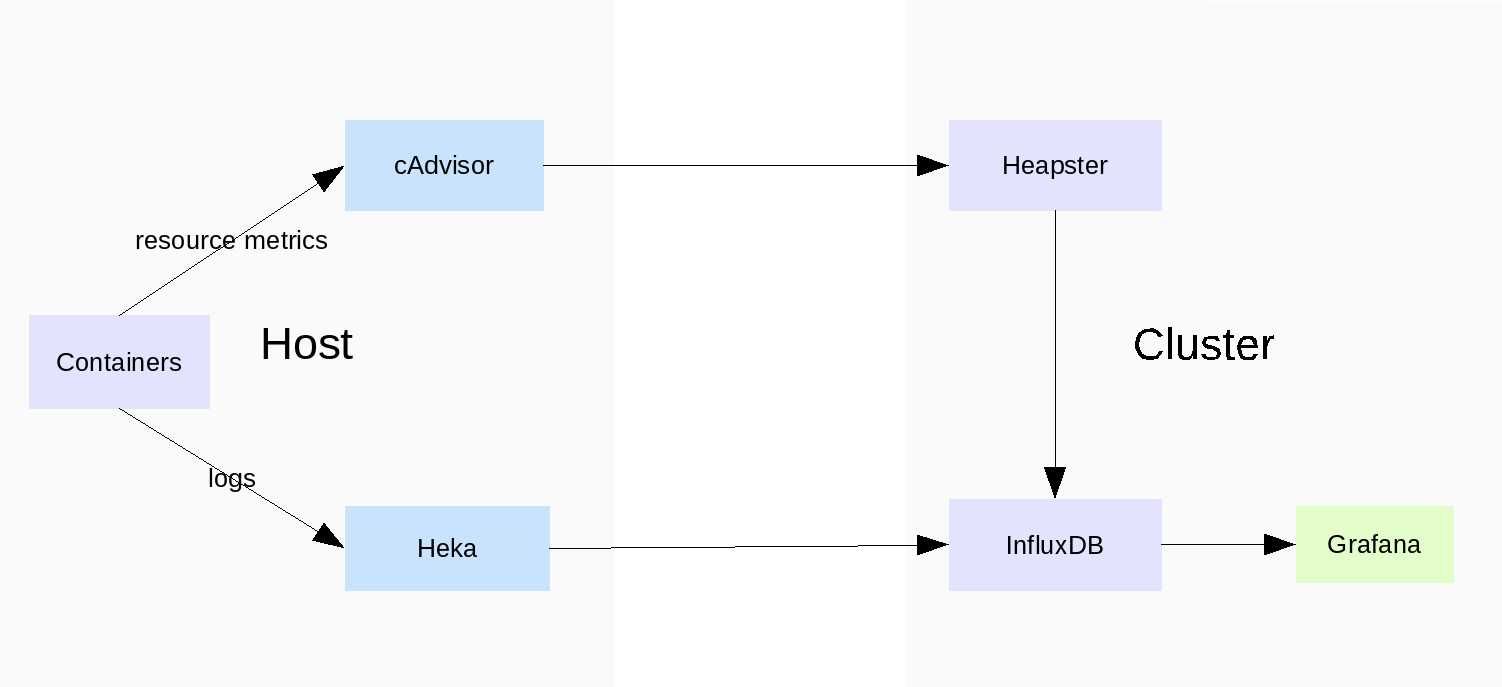
\includegraphics{media/ch6-overview.png}
\caption{Overview of monitoring system}
\end{figure}

The monitoring stack is deployed as an unique application, and includes
\texttt{ReplicationController}s, \texttt{Service}s but also
\texttt{Route}s for external reachability:

\section{Time-Series Storage}\label{time-series-storage}

InfluxDB is a distributed time-series database that fits well since it
doesn't need a predefined schema for data, it's horizontally scalable
in the NoSQL way, support native data replication and include a familiar
SQL-like language, InfluxQL\footnote{https://influxdb.com/docs/v0.8/api/query\_language.html}.

A single metric of a resource could be stored as (in YAML format):

\begin{verbatim}
- 
  name: load_avg
  columns: [ time, app, value ]
  points: [[ 1400425342091, pod_name, 0.8 ]]
\end{verbatim}

Instead a line of log could be stored as:

\begin{verbatim}
-
  name: log_lines
  columns: [ time, app, line ]
  points: [[ 1400425947368, pod_name, "some useful log info" ]]
\end{verbatim}

This is only a very basic example, of course additional columns could increase the usefulness of archived data.

In OpenShift, InfluxDB runs as component of monitoring application, and
is composed by a \texttt{replicationController} and a \texttt{service}:

\section{Resource Gathering}\label{resource-gathering}

Kubernetes comes with built-in cAdvisor in Kubelet, for resource metrics gathering, such as CPU, RAM, I/O, network, etc.

Heapster is the Kubernetes cluster monitoring system, that gather metrics from nodes and send them to InfluxDB.

The exported metrics are:
\begin{itemize}

\item
  uptime: Number of milliseconds since the container was started;
\item
  cpu/usage: Cumulative CPU usage on all cores;
\item
  cpu/limit: CPU limit in millicores;
\item
  memory/usage: Total memory usage;
\item
  memory/working\_set: Total working set usage. Working set is the
  memory being used and not easily dropped by the kernel;
\item
  memory/limit: Memory limit;
\item
  memory/page\_faults: Number of page faults;
\item
  memory/major\_page\_faults: Number of major page faults;
\item
  network/rx: Cumulative number of bytes received over the network;
\item
  network/rx\_errors: Cumulative number of errors while receiving over
  the network;
\item
  network/tx: Cumulative number of bytes sent over the network;
\item
  network/tx\_errors: Cumulative number of errors while sending over the
  network;
\item
  filesystem/usage: Total number of bytes consumed on a filesystem;
\item
  filesystem/limit: The total size of filesystem in bytes.
\end{itemize}

While the exported labels are:

\begin{itemize}
\item
  hostname: Hostname where the container ran;
\item
  host\_id: Identifier specific to a host. Set by cloud provider or user;
\item
  container\_name: User-provided name of the container or full container
  name for system containers;
\item
  pod\_name: The name of the pod;
\item
  pod\_id: The unique ID of the pod;
\item
  pod\_namespace: The namespace of the pod;
\item
  namespace\_id: The UID of namespace of the pod;
\item
  labels: Comma-separated list of user-provided labels;
\item
  resource\_id: Identifier(s) specific to a metric.
\end{itemize}

Heapster is deployed as \texttt{replicationController}, a \texttt{service} and a \texttt{route}.

\section{Log Processing}\label{log-processing}

\textit{Heka} is a framework developed by Mozilla for easy data collection and processing. Heka is modular and supports mainly 6 different type of plugins: inputs, splitters, decoders, filters, encoders and outputs. The first 3 are for gather and parse incoming data to \textit{Heka Message} standard, the filters parse all these messages and the later 2 is for encoding and sending data somewhere else, for storing or further processing.

Heka permits to logs parsing, filtering, structuring them and send to InfluxDB. In this example will be used Gasista Felice's NGiNX component for generating logs and \textit{boom} for doing a lot of requests.

\begin{figure}[htbp]
\centering
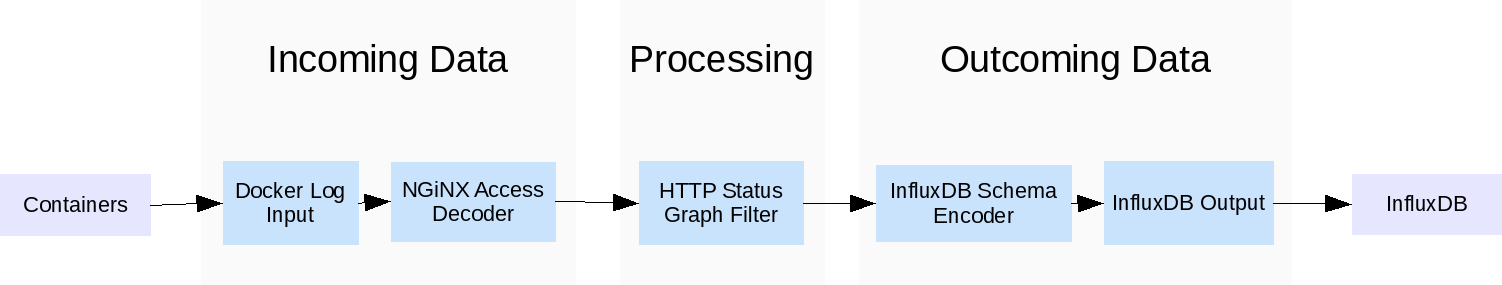
\includegraphics{media/ch6-heka.png}
\caption{The Heka Data Flow}
\end{figure}

As shown in figure 6.2, the input part is composed by the \textit{Docker Log Input}, build on top of \textit{Logspout} that acquires stdout/stderr of running containers from the Docker Engine Unix socket, and \textit{NGiNX access} and \textit{error decoders}.  Filtering consist of \textit{HTTP Status Graph} that filter NGiNX access logs and generate an HTTP response code based graph.  Finally the output part is composed by encoding in \textit{InfluxDB schema} and sending data to \textit{InfluxDB HTTP APIs}.

Heka is deployed on top of OpenShift as a simple \texttt{replicationController}.

\section{Data Visualization}\label{data-visualization}

Grafana is a metrics dashboard and graph editor, born as fork of Kibana in the beginning of 2014.

\begin{figure}[htbp]
\centering
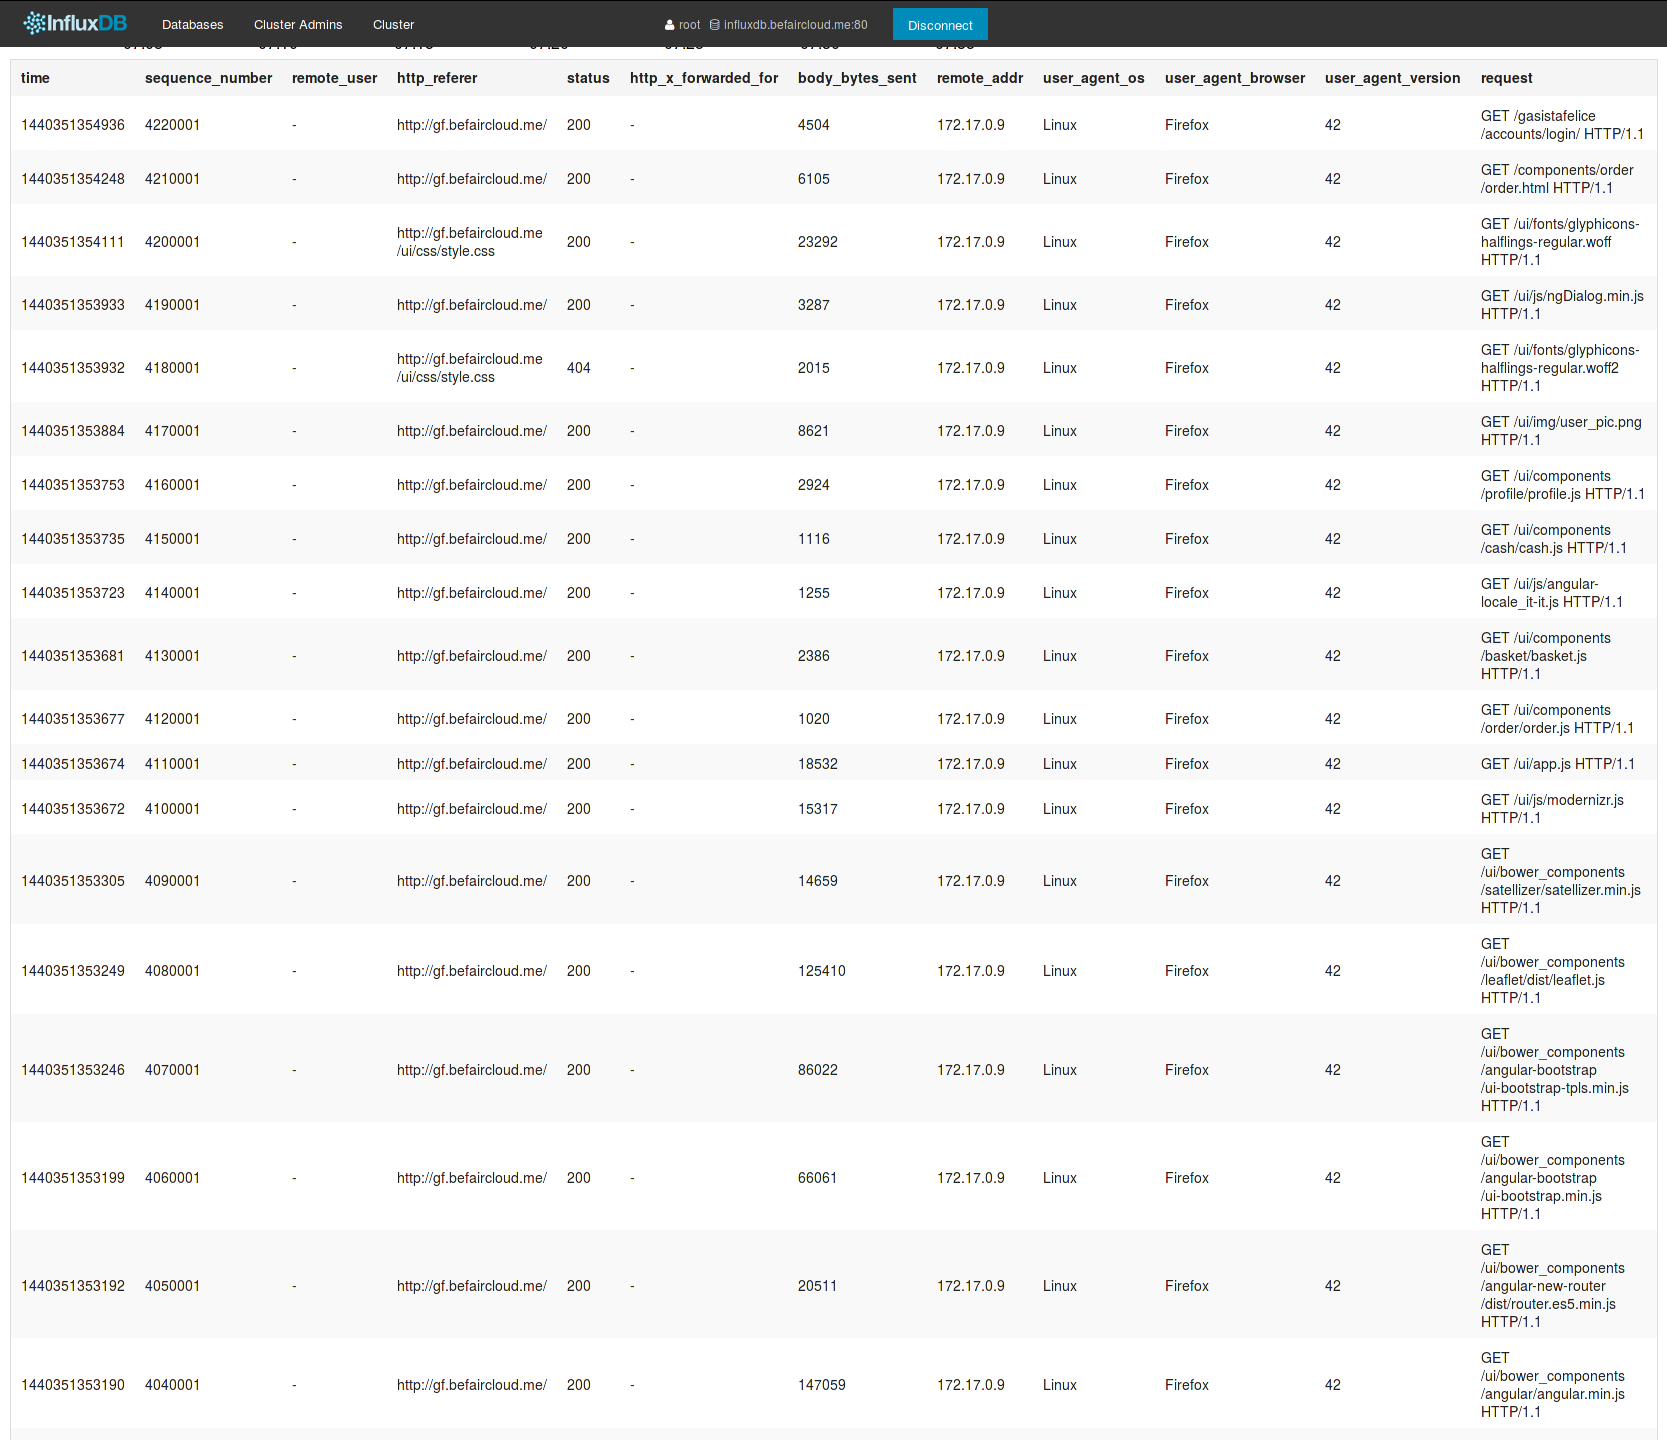
\includegraphics{media/ch6-influxdb.png}
\caption{InfluxDB logs dashboard}
\end{figure}

Figure 6.3 shows structured logs from InfluxDB dashboard, that have been queried from Grafana dashboard.

The first 2 graphs in Grafana dashboard show data derived from logs processing, while the last 2 from Heapster:

\begin{verbatim}
# Show the network traffic
select mean(body_bytes_sent) from "nginx.access"

# Show the success and failure responses
select count(status) from "nginx.access" where status < 400
select count(status) from "nginx.access" where status >= 400

# Show the CPU load of backend
select derivative(value) from "cpu/usage_ns_cumulative" \
    where container_name="back"

# Show the memory usage of backend
select value from "memory/usage_bytes_gauge" \
    where container_name="back"
\end{verbatim}

Figure 6.4 shows the graphical results of these queries.

\begin{figure}[htbp]
\centering
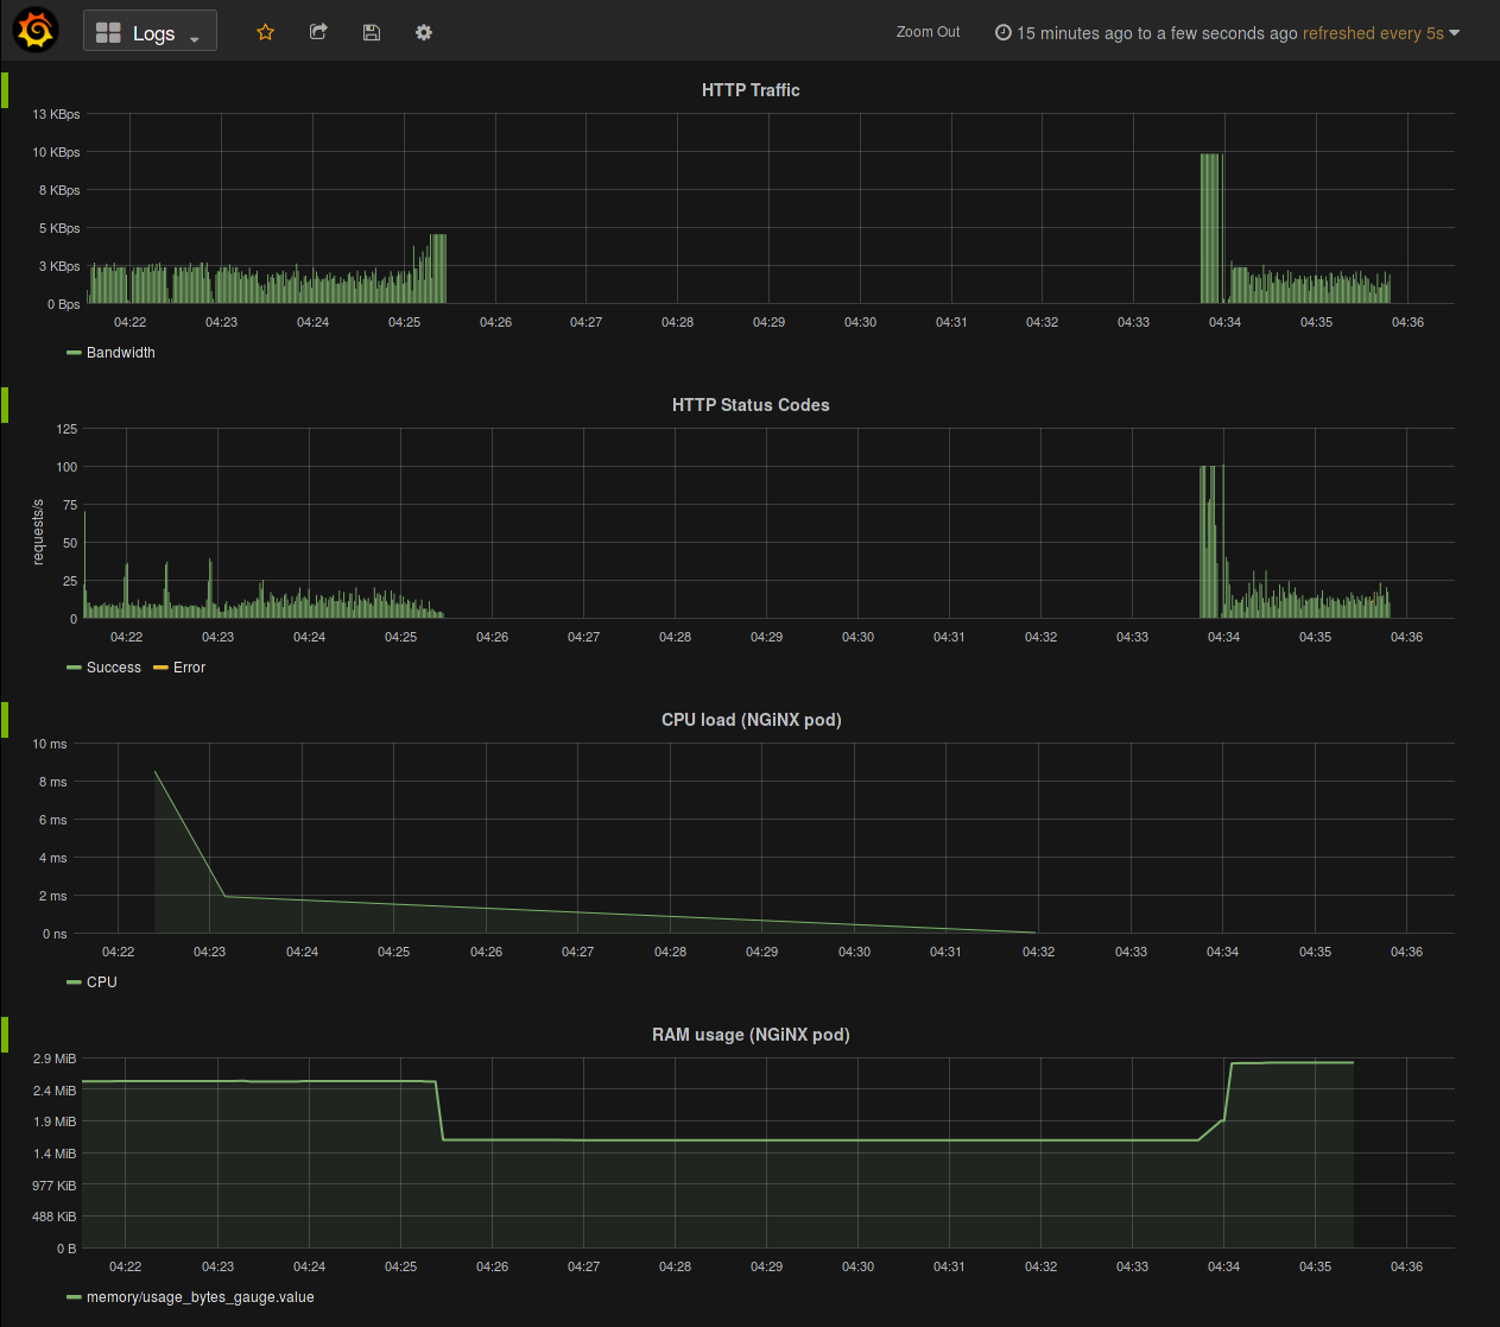
\includegraphics{media/ch6-grafana.png}
\caption{Grafana dashboard}
\end{figure}

Grafana is deployed with a \texttt{replicationController}, a \texttt{Service} and a \texttt{Route} in order to be reached from the external.